% -*- TeX -*- -*- UK -*- -*- Soft -*-"

\chapter{Setting DVIPS}


\section{PostScript Specials and Security}

The issue discussed here became evident in Miktex 2.5, but could also apply to any other application that uses DVIPS.  The problem presented itself as an inability of YAP to preview some DVI pages.


As from Version 5.95b DVIPS does not support 'unsecure' path names, such as \\
- absolute path names (like C:/temp/eurotour.eps)\\
- parent-relative path names (like ../../temp/eurotour.eps)\\
which means that the following will not work:\\
\verb+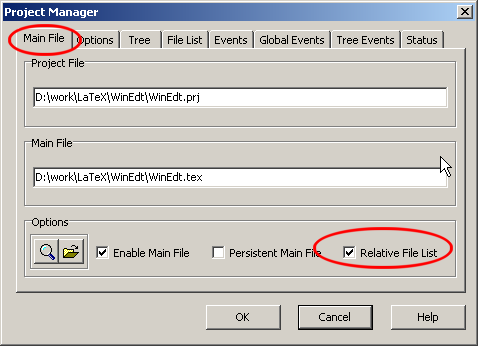
\includegraphics[bb= 0 0 512 387,scale=0.7]{eps/projectmanager.png}+

YAP complains with a message similar to:
{\small
\begin{verbatim}
MiKTeX Problem Report
Message: The page could not be rendered.
Data: This is dvips(k) 5.95b Copyright 2005 Radical Eye Software (www.radicaleye.com)
' TeX output 2006.05.28:2135' ->
<tex.pro><texps.pro><special.pro>. <cmbx12.pfb><cmr10.pfb>[2<eurotour.eps>
C:\Program Files\MiKTeX 2.5\miktex\bin\dvips.exe:
Could not find figure file c:/temp/eurotour.eps; continuing
\end{verbatim}
}

On Cristian Schenk's page he states:\\
(\verb+http://dojo.miktex.org/blogs/christian_schenk/archive/2006/03/06/328.aspx+)

{\small
\begin{verbatim}
It would be possible to break these security rules by
- using the Dvips option -R0
- by specifying z0 in the Dvips configuration file
\end{verbatim}
}

Schenk offered to implement the first option with a future release of YAP, but as of version 2.7 is still is not implemented.  Our recourse is then to implement the second option ourselves.

On my PC,the DVIPS config file, \verb"config.ps", is located at the following location:

\verb+C:\Program Files\MiKTeX 2.7\dvips\config+

In this file, find these lines:

\begin{verbatim}
% z1 is "secure", i.e., inhibits execution of `shell commands` in
% \specials.  Dvips allows this by default.
z1
\end{verbatim}

and change it to this:

\begin{verbatim}
% z1 is "secure", i.e., inhibits execution of `shell commands` in
% \specials.  Dvips allows this by default.
z0
\end{verbatim}

At the top of the config file it instructs us to use \verb"initexmf" to change this file, but I could not find an easy way to do this, so I just manually edited \verb"config.ps".  It seems to work.



